\documentclass[svgnames]{article}
\usepackage[utf8]{inputenc}
\usepackage{amsmath}
\usepackage{amssymb}
\usepackage{mathrsfs}
\usepackage{mathtools}
\newtheorem{mydef}{Given}
\newtheorem{mytheorem}{Theorem}
\usepackage{enumitem}
\usepackage{venndiagram}
\usepackage{smartdiagram}
\usepackage{caption}
\usepackage{subcaption}
%\usepackage[framed,numbered,autolinebreaks,useliterate]{mcode}
\usepackage{pgfplots}
%\usepackage{tkiz}
\usepackage{listings}
\definecolor{dkgreen}{rgb}{0,0.6,0}
\definecolor{gray}{rgb}{0.5,0.5,0.5}
\definecolor{mauve}{rgb}{0.58,0,0.82}
\usepackage{float}
\usepackage{graphicx}
\graphicspath{ {./images/} }

\lstset{ %
  language=R,                     % the language of the code
  basicstyle=\footnotesize,       % the size of the fonts that are used for the code
  numbers=left,                   % where to put the line-numbers
  numberstyle=\tiny\color{gray},  % the style that is used for the line-numbers
  stepnumber=1,                   % the step between two line-numbers. If it's 1, each line
                                  % will be numbered
  numbersep=5pt,                  % how far the line-numbers are from the code
  backgroundcolor=\color{white},  % choose the background color. You must add \usepackage{color}
  showspaces=false,               % show spaces adding particular underscores
  showstringspaces=false,         % underline spaces within strings
  showtabs=false,                 % show tabs within strings adding particular underscores
  frame=single,                   % adds a frame around the code
  rulecolor=\color{black},        % if not set, the frame-color may be changed on line-breaks within not-black text (e.g. commens (green here))
  tabsize=2,                      % sets default tabsize to 2 spaces
  captionpos=b,                   % sets the caption-position to bottom
  breaklines=true,                % sets automatic line breaking
  breakatwhitespace=false,        % sets if automatic breaks should only happen at whitespace
  title=\lstname,                 % show the filename of files included with \lstinputlisting;
                                  % also try caption instead of title
  keywordstyle=\color{blue},      % keyword style
  commentstyle=\color{dkgreen},   % comment style
  stringstyle=\color{mauve},      % string literal style
  escapeinside={\%*}{*)},         % if you want to add a comment within your code
  morekeywords={*,...}            % if you want to add more keywords to the set
} 


%\renewcommand{\theenumi}{\Alph{enumi}}
\newenvironment{amatrix}[1]{%
  \left(\begin{array}{@{}*{#1}{c}|c@{}}
}{%
  \end{array}\right)
}

\newenvironment{tolerant}[1]{%
  \par\tolerance=#1\relax
}{%
  \par
}


\pgfmathdeclarefunction{gauss}{2}{%
  \pgfmathparse{1/(#2*sqrt(2*pi))*exp(-((x-#1)^2)/(2*#2^2))}%
}


\title{Statistical methods: Homework 9}
\author{Cameron McIntyre}
\date{\today}

\begin{document}

\maketitle

\section{6.2.2}

An herbalist is experimenting with juices extracted from berries and roots that may have the ability to affect the Stanford-Binet IQ scores of students afflicted with mild cases of attention deficit disorder (ADD). A random sample of twenty-two children diagnosed with the condition have been drinking Berry Smart daily for two months. Past experience suggests that children with ADD score an average of 95 on the IQ test with a standard deviation of 15. If the data are to be analyzed using the $\alpha = 0.06$ level of significance, what values of $\Bar{y}$ would cause $H_0$ to be rejected? Assume that $H_1$ is two-sided.

\subsection*{Answer:}
We need to find the critical value of a 2 sided test with $\alpha=.06$. We should fin $z_{.03}$ to represent both extremes. 
Using R Software Package:

\begin{lstlisting}
> qnorm(.03)
[1] -1.880794
> qnorm(1-.03)
[1] 1.880794
\end{lstlisting}

We now calculate our test statistics.
For the right tailed rejection criteria,
$$\frac{\bar{y}-95}{\frac{15}{\sqrt{22}}}>1.88 \leftrightarrow \bar{y} > 101.0123$$
101.01 represents the upper critical value for rejection
For the left tailed rejection criteria,
$$\frac{\bar{y}-95}{\frac{15}{\sqrt{22}}}<-1.88 \leftrightarrow \bar{y} < 88.98774$$
88.987 represents the lower critical value for rejection

\section{6.2.10}
 As a class research project, Rosaura wants to see whether the stress of final exams elevates the blood pressures of freshmen women. When they are not under any untoward duress, healthy eighteen-year-old women have systolic blood pressures that average 120mm Hg with a standard deviation of 12mmHg. If Rosaura finds that the average blood pressure for the fifty women in Statistics 101 on the day of the final exam is 125.2, what should she conclude? Set up and test an appropriate hypothesis.
\subsection{Answer}
We are looking for the right tailed rejection region. The critical value for 95\% on the normal distribution is 1.644854.

\begin{center}
\textbf{H$_0:$} Blood pressure on test day is the same as any other day. 
\newline
\textbf{H$_1:$} Blood pressure is elevated on test day. 
\end{center}
 $$\frac{125.2-120}{\frac{12}{\sqrt{50}}}> 1.644854 \leftrightarrow 3.064129 > 1.64 $$
 
 Therefore we reject the null hypothesis and accept $H_1$, meaning that the blood pressure is significantly elevated on test day. 

\section{6.3.6}
Among the early attempts to revisit the death postponement theory introduced in Case Study 6.3.2 was an examination of the birth dates and death dates of three hundred forty-eight U.S. celebrities (144). It was found that sixteen of those individuals had died in the month preceding their birth month. Set up and test the appropriate $H_0$ against a one-sided $H_1$. Use the 0.05 level of significance.

\subsection*{Answer:}

So lets set up our Hypotheses;
\begin{center}
\textbf{H$_0$:} There rate of death in the month preceding a celebrity's death is $\frac{1}{12}$.
\newline
\textbf{H$_1$:} There rate of death in the month preceding a celebrity's death is lower than $\frac{1}{12}$
\end{center}

Our critical value is -1.644854.
\newline
Our test statistic is:
$$ \frac{16-\frac{1}{12}*348}{\sqrt{348(\frac{1}{12})*(1-\frac{1}{12})}}=-2.521382$$

Since -2.521382 is less than - 1.644, we reject \textbf{H$_0$} and claim that the rate of death of celebrities less significantly less than $\frac{1}{12}$.

\section{6.4.4}
Construct a power curve for the $\alpha = 0.05$ test of $H_0: \mu = 60$ versus $H_1: \mu \neq 60$ if the data consist of a random sample of size 16 from a normal distribution having $\sigma = 4$.
\subsection*{Answer:}
We use R to sort this out. 

\begin{lstlisting}
#Construct a power curve for the ? = 0.05 test of 
#H0:?=60 versus H1:?=60 if the data consist of a
#random sample of size 16 from a normal distribution having ? = 4.
sig_left = qnorm(.025)
sig_right = -qnorm(.025)

reject_left = sig_left*(4/4)+60
reject_right = sig_right*(4/4)+60

rnge = 500:700/10

draw_target <- function(x) {
  return(1- (pnorm((reject_right-x)/(4/4)) - pnorm((reject_left-x)/(4/4))))
  }

plot(rnge, draw_target(rnge))
\end{lstlisting}
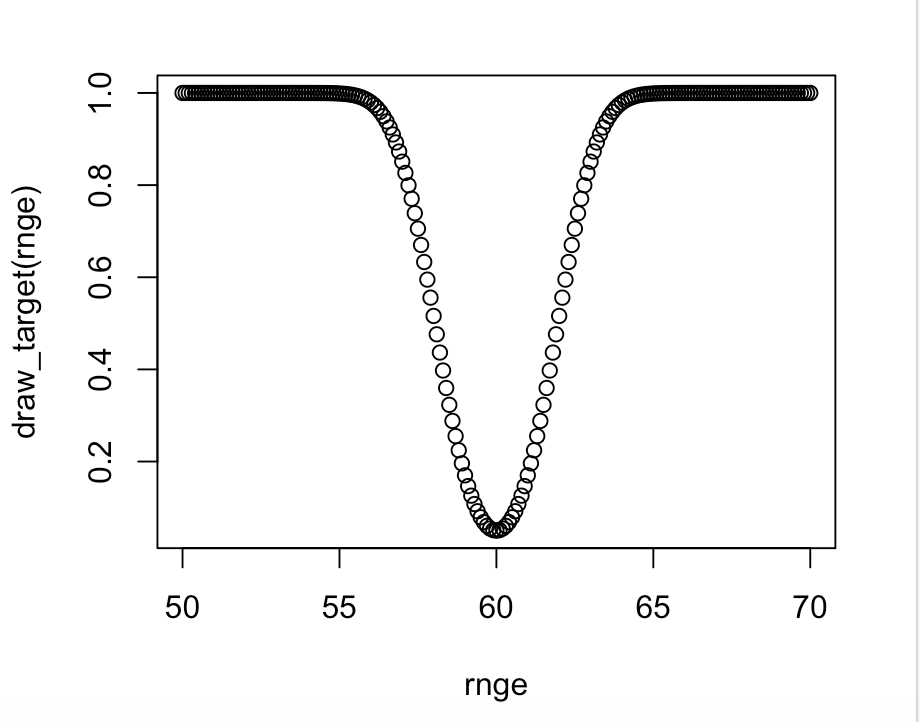
\includegraphics[scale=1.05]{PowerCurve}

\section{6.4.18}
An experimenter takes a sample of size 1 from the Poisson probability model, $p_X(k) = e^{-\lambda}\lambda^k/k!, k = 0, 1, 2,... $, and wishes to test

\begin{align*}
    H_0&: \lambda =6\\
    &\text{versus}\\
    H_1 &: \lambda < 6
\end{align*}

by rejecting $H_0$ if $k \leq 2$.

\begin{enumerate}[label = (\alph*)]
    \item Calculate the probability of committing a Type I error. 
    \subsection*{Answer:}
    $$P(Type\ 1\ Error)=P(Reject\ H_0|H_0\ is\ true)=P(k=0)+P(k=1)+P(k=2)$$
    $$P(Type\ 1\ Error)=0.002478752 + 0.014872513 + 0.044617539=0.062$$
    \item Calculate the probability of committing a Type II error when $\lambda = 4$.
    \subsection*{Answer:}
    $$P(Type\ 2\ Error)=P(Accept\ H_0|H_0\ is\ False\ and \ \lambda=4)=P(k > 2 | \lambda=4)$$
    $$P(Type\ 2\ Error) = 1 - P(k \leq 2)= 1- 0.0183 + 0.0732 + 0.1465 = 0.7618$$
\end{enumerate}

\section{6.5.2}
 Let $y_1, y_2,..., y_{10}$ be a random sample from an exponential pdf with unknown parameter $\lambda$. Find the form of the GLRT for $H_0: \lambda = \lambda_0$ versus $H_1: \lambda \neq \lambda_0$. What integral would have to be evaluated to determine the critical value if $\alpha$ were equal to 0.05?
\subsection*{Answer:}
\begin{center}
\textbf{H$_0$} $\lambda = \lambda_{0}$ And 
\textbf{H$_1$} $\lambda \neq \lambda_{0}$
\end{center}

$$L_p(\omega)=\Pi_{i=1}^{n}\lambda e^{\lambda_{X_{i}}} = \lambda^ne^{-\lambda n \bar{x}}$$

Forming the ratio of likelihoods and knowing the MLE for the exponential distribution $\hat{\lambda}=\frac{1}{\bar{x}}$,
$$\lambda_{ratio}=\frac{L(\omega)}{L(\Omega)}=\frac{ \lambda_{0}^ne^{-\lambda_{0} n \bar{x}}}{\hat{\lambda}^ne^{-\hat{\lambda} n \bar{x}}} $$

So the integral we have to solve is:

$$\int^{\lambda = y }_{0} \lambda_{0}^n\hat{\lambda}^{-n}e^{({+\hat{\lambda}-\lambda_{0})* n \bar{x}}} d\lambda_{0} =.05$$
Now we substitute our values and simplify.
$$\int^{\lambda = y }_{0} \lambda_{0}^{10}e^{-\lambda_{0}\sum x_i} d\lambda_{0} =.05 $$

\section{7.3.2}
 Find the moment-generating function for a chi square random variable and use it to show that $E(\chi_n^2) = n$ and Var$(\chi_n^2) = 2n$. 

\subsection*{Answer:}
A chi square random variable is the sum of squared normal random variables, and is a special case of the gamma distribution. so we find the MGF for this case of the gamma distribution. 

$$Mg(t)=E[e^{xt}]=\int_{0}^{\infty}e^{tx}\frac{1}{2^{\frac{n}{2}}\Gamma(\frac{n}{2})}e^{\frac{n}{2}-1}x^{\frac{x}{2}}=(1-2t)^{-\frac{n}{2}}$$

Then,
$$E[x]=M'(t)=\frac{d}{dt}(1-2t){-\frac{n}{2}}=\frac{n}{2}(1-2t)^{-\frac{n}{2}-1}*-2\Big|_{t=0}=n$$

And,
$$E[x^2]=\frac{d}{dt}n(1-2t)^{-\frac{n}{2}-1}=\Big[-( \frac{n^2}{2}-n)(1-2t)^{\frac{n}{2}-2}\Big]*-2\Big|_{t=0}=n^2+2n$$

Finally:
$$Var[X]=E[X^2]-E[X]^2=n^2+2n - n^2= 2n$$


\section{7.3.7}
Use Appendix Table a.4 to find
\begin{enumerate}[label = (\alph*)]
\item $F_{.50,6,7}$
\item $F_{.001,15,5}$
\item $F_{.90,2,2}$
\end{enumerate}
\subsection*{Answer:}

\begin{enumerate}[label = (\alph*)]
\item $F_{.50,6,7}$
\newline
Using R:
\begin{lstlisting}
> qf(.5, df1=6,df2=7)
[1] 0.9833387
\end{lstlisting}
So,  $F_{.50,6,7} = 0.9833387$

\item $F_{.001,15,5}$
\begin{lstlisting}
> qf(.001, df1=15,df2=5)
[1] 0.1321459
\end{lstlisting}
So,  $F_{.001,15,5} = 0.1321459$

\item $F_{.90,2,2}$
\begin{lstlisting}
> qf(.90, df1=2,df2=2)
[1] 9
\end{lstlisting}
So,  $F_{.9,2,2} = 9$
\end{enumerate}


\section{7.4.2}
What values of x satisfy the following equations? 
\begin{enumerate}[label = (\alph*)]
\item $P(-x\leq T_{22} \leq x) = 0.98$
\item $P(T_{13} \geq x) = 0.85$
\item $P(T_{26} < x) = 0.95$
\item $P(T_{2} \geq x) = 0.025$
\end{enumerate}
\subsection*{Answer:}
\begin{enumerate}[label = (\alph*)]
\item $P(-x\leq T_{22} \leq x) = 0.98$
\newline
We use R.
\begin{lstlisting}
> qt(.99, df=22)
[1] 2.508325
> pt(2.508325, df=22)-pt(-2.508325, df=22)
[1] 0.98
\end{lstlisting}
x=2.508325
\newline
Therefore $P(-2.508325\leq T_{22} \leq 2.508325) = 0.98$

\item $P(T_{13} \geq x) = 0.85$

$$P(T_{13} \geq x) =  1- P(T_{13} < x) = 1 -  .15 $$

We use R.
\begin{lstlisting}
> qt(.15, df=13)
[1] -1.079469
\end{lstlisting}
x = -1.079469
\newline
Therefore $P(T_{13} \geq -1.079469) = 0.85$

\item $P(T_{26} < x) = 0.95$
\newline
We use R.
\begin{lstlisting}
> qt(.95, df=26)
[1] 1.705618
\end{lstlisting}
x = 1.705618
\newline
Therefore $P(T_{26} < 1.705618) = 0.95$


\item $P(T_{2} \geq x) = 0.025$

$$P(T_{2} \geq x) = 0.025 \leftrightarrow P(T_{2} \geq x) = 1 - .975 $$
\newline
We use R.
\begin{lstlisting}
> qt(.975, df=2)
[1] 4.302653
\end{lstlisting}
x = 4.302653
\newline
Therefore $P(T_{2} \geq 4.302653) = 0.025$
\end{enumerate}

\section{7.4.14}

Revenues reported last week from nine boutiques franchised by an international clothier averaged \$59,540 with a standard deviation of \$6860. Based on those figures, in what range might the company expect to find the average revenue of all of its boutiques?

\subsection*{Answer:}
Confidence interval at $\alpha=.95$ and t distribution with 8 df:

$$(\bar{y}-t_{\frac{\alpha}{2},8}*\frac{s}{\sqrt{n}},\bar{y}-t_{\frac{1-\alpha}{2},8}*\frac{s}{\sqrt{n}})=(59540-5273.05, 59540+5273.05)$$

$$(54266.95,64813.05)$$

Therefore we can be 95 \% certain the revenues are within this range. 

\section{7.4.20}

In addition to the Shoshoni data of Case Study $7.4.2$, a set of rectangles that might tend to the golden ratio are national flags. The table below gives the width-to-length ratios for a random sample of the flags of thirty-four countries. Let $\mu$ be the width-to--length ratio for national flags. At the $\alpha = 0.01$ level, test $H_0 : \mu = 0.618$ versus $H_1 : \mu = 0.618$.

\begin{table}[h!]
\centering
 \begin{tabular}{c c} 
 \hline
Country & Ratio Width to Height \\ [0.5ex] 
 \hline
 Afghanistan	&	0.500	\\
Albania	&	0.714	\\
Algeria	&	0.667	\\
Angola	&	0.667	\\
Argentina	&	0.667	\\
Bahamas	&	0.5	\\
Denmark	&	0.757	\\
Djibouti	&	0.553	\\
Ecuador	&	0.5	\\
Egypt	&	0.667	\\
El Salvador 	&	0.6	\\
Estonia	&	0.667	\\
Ethiopia	&	0.5	\\
Gabon	&	0.75	\\
Fiji	&	0.5	\\
France	&	0.667	\\
Honduras	&	0.5	\\
Iceland	&	0.72	\\
Iran	&	0.571	\\
Israel	&	0.727	\\
Laos	&	0.667	\\
Lebanon	&	0.667	\\
Liberia	&	0.526	\\
Macedonia	&	0.5	\\
Mexico	&	0.571	\\
Monaco	&	0.8	\\
Namibia	&	0.667	\\
Nepal	&	1.25	\\
Romania	&	0.667	\\
Rwanda	&	0.667	\\
South Africa	&	0.667	\\
St Helena	&	0.5	\\
Sweden	&	0.625	\\
United Kingdom	&	0.5	\\
 [1ex] 
 \hline
 \end{tabular}
\end{table}
\subsection*{Answer}
$$s = \sqrt{\frac{1}{n(n-1)}n\Big( \sum y_i^2 - (\sum y_1)^2 \Big)}$$
$$s = .14$$
Degrees of freedom is 33, and our t table values are $\alpha_{.005,33}= -2.733$ and  $\alpha_{.995,33}= 2.733$. If t is outside of (-2.733, 2.733) we reject.

$$t= \frac{\bar{y} - \mu}{\frac{s}{\sqrt{n}}}=\frac{.64-.618}{\frac{.14}{\sqrt{34}}}=.917$$
Since .917 is in (-2.733, 2.733), we do not reject $H_0$.

\section{7.5.8}
A random sample of size $n = 19$ is drawn from a normal distribution for which $\sigma^2 = 12.0$. In what range are we likely to find the sample variance, $s^2$? Answer the question by finding two numbers $a$ and $b$ such that:

$$P(a\leq S^2 \leq b) = .95$$

\subsection*{Answer:}
$$P(\chi_{\frac{\alpha}{2}, n-1}<\frac{(n-1)S^2}{\sigma^2}<\chi_{1 -\frac{\alpha}{2}, n-1}) = 1- \alpha $$
$$P(\frac{\chi_{.025, 18}\sigma^2}{(n-1)}<S^2<\frac{\chi_{.975, 18}\sigma^2}{(n-1)}) = .95 $$
Substituting our values with, $\chi_{.025, 18} = 8.230746$ and $\chi_{.975, 18} = 31.52638$.

$$P(\frac{8.230746*12}{18}<S^2<\frac{31.52638*12}{18}) = .95 \leftrightarrow P(5.487<S^2<21.01759) = .95 $$ 

So a=5.487 and b = 21.01759.

\section{7.5.16}

When working properly, the amounts of cement that a filling machine puts into 25-kg bags have a standard deviation ($\sigma$) of 1.0 kg. In the next column are the weights recorded for thirty bags selected at random from a day's production. Test $H_0: \sigma^2 = 1$ versus $H_1: \sigma^2 > 1$ using the $\alpha = 0.05$ level of significance. Assume that the weights are normally distributed.

\begin{table}[h!]
\centering
 \begin{tabular}{c c c c c} 
 \hline
26.18 & 25.30  & 25.18  & 24.54  & 25.14 \\
24.22 &  26.48  & 23.97 &  25.83  & 25.05 \\
24.22  & 24.49 &  25.68  & 26.01  & 25.50 \\
25.44 & 24.49 & 25.01 & 25.12 & 25.67\\
26.24 & 25.46 & 25.01 & 24.71 & 25.27\\
25.84 &26.09& 25.21& 26.04 & 25.23 \\
 \hline
 \end{tabular}
\end{table}

\textbf{Answer:}

$$s^2 = \frac{n\sum Y_i^2 - (\sum Y_i)^2}{n(n-1)}=.425$$

Our critical value $\chi_{.975,29}=42.557$

$$\frac{(n-1)s^2}{\sigma^2}=\frac{29*.425}{1}= 12.32$$

So, since 13.32< 42.557, we do not reject the null hypothesis. 

\end{document}
